\chapter{Thermal conductivity simulations of Silica glass}

\LEnote{*** INTRODUCTION, STATO DELL'ARTE ***}

\paragraph{Thermal conductivity of glasses}
Thermal conductivity of glass systems is a fundamental property for many industrial and technological applications, \emph{e.g.} heat management in electronic devices, windows for green architectures.
However, ``thermal conductivity represents largely explored territories, ripe for new research efforts'' [J.Mauro...]\cite{MauroFM14,Mauro2014}. The understanding of thermal conductivity and its structural origin in glasses has been greatly overlooked in the literature. 

\paragraph{Vitreous silica}
Vitreous silica has been the subject of significant research efforts in the last decades, due to is many technological applications that range from thermal insulation to laser engineering, semiconductor fabrication, and optical communication.
In particular, thanks to its excellent UV transparency, mechanical stability, and chemical durability, silica can be used in many optical applications, such as the diffractive elements and the protective windows of the optics assemblies of inertial confinement fusion facilities. In these facilities, extremely intense nanosecond laser pulses are used and can seriously challenge the durability the optical glasses. It is indeed well established that the small defects or impurities of the glass may cause local lattice heating and melting, resulting in damage craters that will rapidly degrade its optical performance \cite{Miller2004,Canaud2004,Miller2010,Chambonneau2014,Kuzuu1999,Stuart1995,Wong2006,Carr2010,Saito2000}. Moreover, these local damages can be mitigated by using pulsed laser treatments that increase the damage sites to temperatures of $2000-5000\un{K}$ in $10^{-9}$ to $10^{-12}\un{s}$ and partially restore the desired optical properties \cite{Soules2011}. 
The interpretation of these types of damage processes require the study of thermal properties and the prediction of the thermal conductivity of silica glass, especially in these extreme conditions that experiments cannot probe.

Furthermore, amorphous silica serves as the basis of multicomponent silica glasses, that are adopted for a wide range of special applications. 
Therefore, predicting the thermal conductivity of silica represent the first step towards the prediction of the thermal conductivity of more complicated glasses, whose components are characterized by a complex chemistry that more is difficult to model.

**Esempio vetri borosilicati ecc**

\LEnote{**AEROGELS: \small Silica aerogel, a highly porous material first synthesized in the
early thirties [1], are currently being produced using a sol–gel process
such as hydrolyzing tetramethoxysilane (TMOS) to form silica and
methanol, and subsequently dried through supercritical drying together
with carbon dioxide [2]. Silica aerogel has several highly desirable
properties including being environmentally safe, having high optical
transmission as well as large thermal resistance [3]. These properties
make silica aerogel very suited for applications such as thermal and
acoustic insulation in buildings and appliances, passive solar energy
collection devices, and dielectrics for integrated circuits [4]. Also, it is a
suitable substitute for chlorofluorocarbon-based plastics in thermal
insulation of refrigerators. The most well-known application was in
Cherenkov radiators [5] as Cherenkov counters. Another crucial characteristic
of aerogels is their extremely low density for a solid, which can
go as low as 0.003 g/cm3
. Comparatively, the density of air is approximately
0.0012 g/cm3
, which is only three times lower than that of the
silica aerogel. This would represent significant weight savings when
used in various monolithic structures. **}

%%%%%%%%%%%%%%%%%%%%%%%%%%%%%%%%%%%%%%%%%%%%%
\section{Classical simulations: sample}
\LEnote{Intro su structure, quench rate, force field.}


\LEnote{**da spostare in sec dopo**}
Thermal conductivity depends on:
\begin{itemize}
    \item Potential
    \item simulation protocol (NEMD, EMD), size effects, quantum effects
    \item structure
    \item quenching
\end{itemize}

\subsection{Force field}

The structure of amorphous silica is made of tetrahedra of SiO$_4$, where silicon is at the center, bonded to 4 oxygen atoms located at the vertexes. Each oxygen, in turn, bridges the tetrahedral corners, bonding between two silicon centers. The variation in orientation of adjacent tetrahedra makes the medium and long range structures disordered, forming a typical glass network.

\begin{figure}
    \centering
    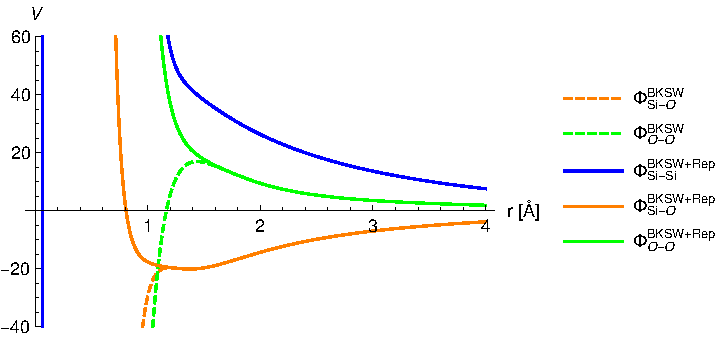
\includegraphics[]{chapters/chapter6/figures/BKSW.pdf}
    \caption{BKS potential with Wolf truncation.}
    \label{fig:BKS-potential}
\end{figure}

One of the most successful force fields for a-SiO$_2$ is the so-called BKS potential \cite{Silica-BKS-1990}. 
The BKS potential was devised by \citeauthor*{Silica-BKS-1990} who fit self-consistent-field Hartree-Fock calculations on small silica clusters, and it has the form...

FORM OF BKS...

TRUNCATION
PARAMETRI USATI (nella sezione risultati)

Despite its simplicity, BKS was showed to predict remarkably well many properties of SiO$_2$, among which its complicated phase diagram \cite{Saika2004}. 
Many other force fields have been used in the literature, ranging from simple two-body potentials like the BKS or re-parametrizations of it \cite{Carre2008}, to polarizable force fields \cite{Tangney2002} and reactive force fields (\emph{e.g.} ReaxFF \cite{Yuan2001}). 
Notwithstanding, the BKS potential is still the mostly adopted force field in classical simulations of a-SiO$_2$, thanks to its ability to reproduce faithful glass structures. 
In the following and in Sec.~\ref{sec:glass-quenching} we are going to summarize how the properties of amorphous silica are reproduced by this potential and others.

\paragraph{Structural properties}
\LEnote{For example...}
\citet{Tian2017} compared the structures of silica obtained from different force fields. They quenched a fully melted silica box of density $\rho=2.2\un{g/cm^3}$ from $5000\un{K}$ to $300\un{K}$ at $5\times 10^{12}\un{K/s}$ in the NVT ensemble. 
The BKS and ReaxFF potentials both generate realistic silica structures \cite{Vollmayr1996,Yuan2001}, with radial distribution functions, neutron structure factors, and coordination numbers that reasonably reproduce the experimental observations.
The radial distribution functions present a first sharp peak at $\sim 1.6\un{\angstrom}$ that corresponds to the Si-O bond length, a second peak at $\sim 2.6\un{\angstrom}$ that represents the distance between two O atoms
\LEnote{**grafici g(r) vedi \cite{Bhattarai2016} o altru**}
\LEnote{**rimuovere TETER va...***}
Si-O: $\sim 1.625\un{\angstrom}$, Si-Si: $\sim 1.62\un{\angstrom}$, Si-O: $\sim 2.65\un{\angstrom}$ \cite{Bhattarai2016}.

The coordination numbers can be used to detect coordination defects, by choosing a cutoff length for Si-O pairs of $\sim 2.0\un{\angstrom}$: BKS reproduces a realistic coordination environment for Si and O, with over $99.6\%$ of atoms being normally coordinated (4-fold Si and 2-fold O). ReaxFF, instead, tends to generate more coordination defects, with $\sim 97.5\%$ of normally coordinated atoms.
Nevertheless, the quenching process largely influences the macroscopic and microscopic properties of the generated glass, so we shall comment more on these point later, in Sec.~\ref{sec:glass-quenching}. 

\begin{description}
    \item[Experimental density] $2.202\un{g/cm^3}$
    \item[Experimental thermal expansion coefficient] $\alpha_v \approx 5.5\times 10^{-7}\un{K^{-1}}$. (CHECK)
\end{description}

\paragraph{VDOS}
\begin{figure}
    \centering
    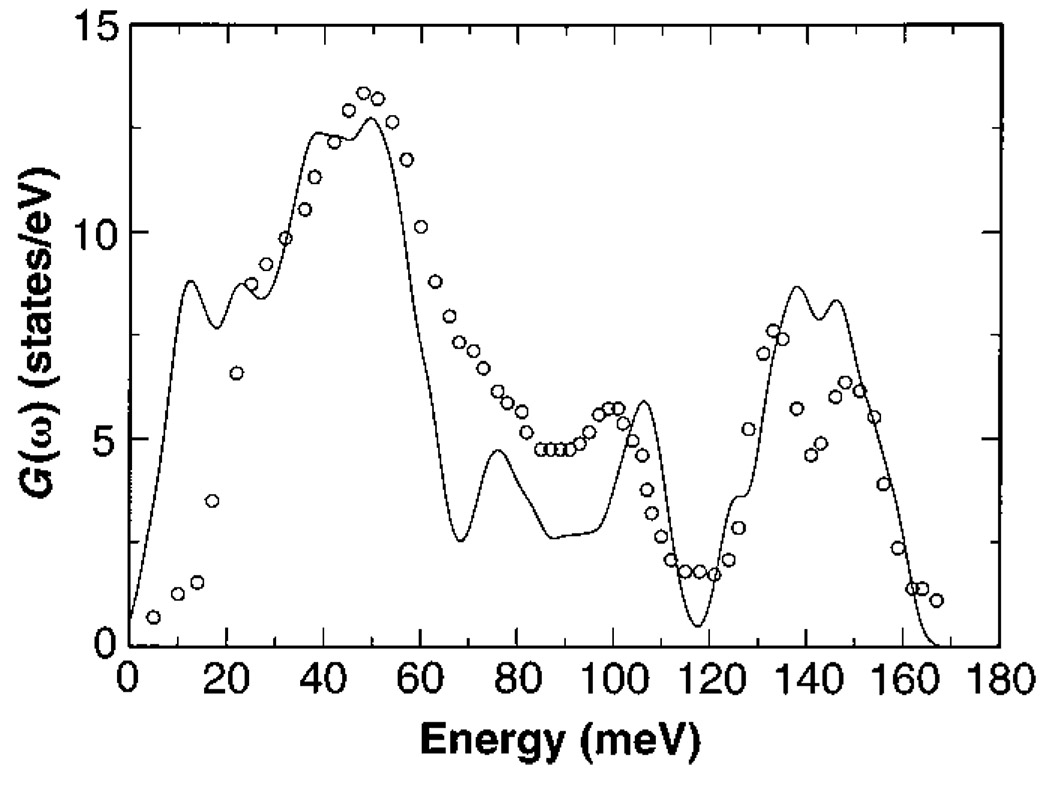
\includegraphics{chapters/chapter6/figures/Sarnthein_Car_abinitio_VDOS_silica-2.jpg}
    \caption{
    Effective vibrational density of states of an a-SiO$_2$ sample of $72$ atoms at experimental density $2.20\un{g/cm^3}$, computed from AI-CPMD simulations within the local density approximation (solid line), compared to neutron scattering data (circles). Reproduced from Ref.~\cite{Sarnthein1997}.}
    \label{fig:silica-vdos-abinitio}
\end{figure}
\begin{figure}
    \centering
    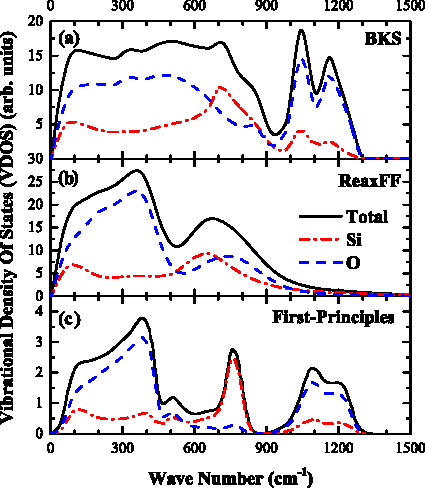
\includegraphics{chapters/chapter6/figures/Tian_VDOS_silica.pdf}
    \caption{
    Total and partial VDOS of a-SiO$_2$ computed for the (a) BKS and (b) ReaxFF, and compared with the (c) first-principle results of \citet{Bhattarai2016}. Adapted from Ref.~\cite{Tian2017}.}
    \label{fig:silica-vdos-classical}
\end{figure}

Besides the structure of the generated sample, what determine the thermal conductivity of the system are its vibrational properties, that are determined by the interaction potential and can be analyzed by the vibrational density of states (VDOS).
Experimentally, the VDOS obtained from neutron scattering shows three significant peaks at about $400\un{cm^-1}$, $800\un{cm^-1}$, and $1100\un{cm^-1}$, that represent the rocking, bending, and stretching modes respectively \cite{Galeener1983}, as shown in Fig.~\ref{fig:silica-vdos-abinitio}.

First principles simulations have shown to successfully reproduce all the principle peaks of the VDOS. \citet{Sarnthein1997} studied a sample of $72$ atoms of a-SiO$_2$ obtained from a quench from the melt with AIMD at experimental density ($2.20\un{g/cm^3}$), within the local density approximation of DFT, and computed the VDOS by diagonalization of the dynamical matrix. Their results, reported in Fig.~\ref{fig:silica-vdos-abinitio}, are in very good agreement with the experiments. The same calculation has been reproduced more recently by \citet{Bhattarai2016} using a $648$-atom model of a-SiO$_2$ (see Fig.\LEnote{Figura articolo Tian, con comparison BKS...}).

Conversely, classical force fields struggle to correctly reproduce the features of the VDOS of a-SiO$_2$. In Fig.~\ref{fig:silica-vdos-classical} we report the VDOS obtained for the BKS and ReaxFF potentials \cite{Tian2017}, compared to an \abinitio calculation \cite{Bhattarai2016}. 
The low-frequency band is dominated by O contributions and agrees well with the results of first-principles simulations and experiments, even though it wrongly elongates up to $600\un{cm^{-1}}$ using the BKS potential. For this model, the modes in the $400-500\un{cm^{-1}}$ range do not agree well with experiment, a sign suggesting that BKS struggles to reproduce correctly the forces over intermediate-range distances \cite{Vollmayr1996}. 
The intermediate-frequency band of \abinitio simulations is dominated by Si contributions and presents an isolated peak at about $800\un{cm^{-1}}$, but this is not reproduced by the BKS potential, while ReaxFF does not account correctly for the contributions of Si and O atoms. 
The high-frequency band, that corresponds to Si-O stretching vibrations, is well reproduced by the BKS potential, but is notably missing in ReaxFF. 
Therefore we can expect that ReaxFF will provide more realistic predictions of thermal conductivity at room temperature, where thermal conduction is mainly contributed by acoustic-like phonon vibrations whose frequencies are typically below $400\un{cm^{-1}}$ \cite{Bhattarai2016}; whereas the BKS potential will probably be more suitable to study high-temperatures cases, where the contribution of stretching vibrations to thermal conduction increases significantly. 


\subsection{Sample preparation}

\subsection{Quenching}  \label{sec:glass-quenching}
The properties of the simulated glass may sensibly depend on the quenching process adopted to generate the virtual sample. 
When a supercooled liquid is cooled down so much that the relaxation times of the system exceed the time scale of the (virtual) experiment, the system will be in a nonequilibrium state and undergo a glass transition, provided it does not crystallize. The obtained glass is a nonequilibrium structure whose properties will generally depend on its production history. The \emph{quenching rate} at which it was cooled will determine its macroscopic and, in particular, microscopic properties \cite{Vollmayr1996}. 
For example, the glass transition temperature computed by simulations is significantly higher than the glass transition temperature observed in the laboratory. 
The time scales reachable by computer simulations are many orders of magnitude shorter than the typical time scales of laboratory experiments, hence the minimum quenching rates attainable in classical MD simulations are of the order of $10^{11}-10^{13}\un{K/s}$, a rate that can only be replicated experimentally by strong laser pulses or ion bombardment \cite{Soules2011}.

\citet{Vollmayr1996} extensively studied the effects of quenching rate on the properties of BKS amorphous silica. They used a sample of $\sim 1000$ atoms at zero pressure, melted it at $7000\un{K}$ and then cooled it down to $0\un{K}$ at different temperature rates $\gamma$, ranging from $10^{12}$ to $10^{15}\un{K/s}$. More recently, \cite{Lane2015} extended their study, reaching cooling rates down to $5\times 10^{9}\un{K/s}$ with microsecond MD simulations of $\sim 13000$ atoms.

\begin{figure}
    \centering
    \subfigure[\label{fig:silica-bks-density-anomaly}]{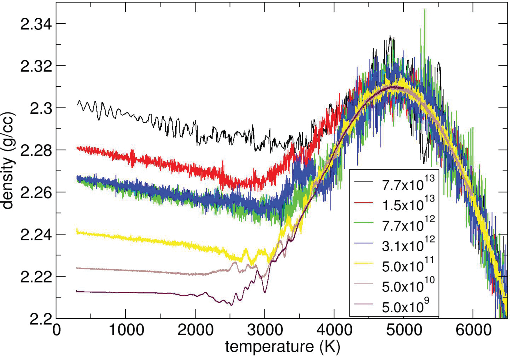
\includegraphics[height=4.6cm]{chapters/chapter6/figures/Lane_density1.pdf}}
    \hfill
    \subfigure[\label{fig:silica-bks-density-temp}]{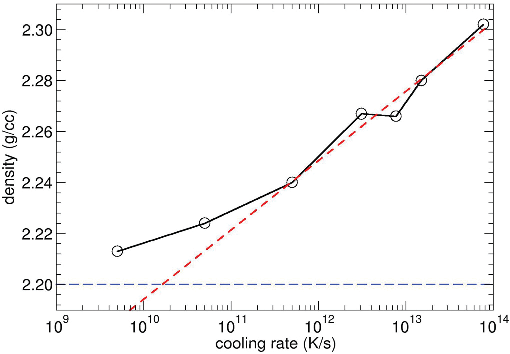
\includegraphics[height=4.6cm]{chapters/chapter6/figures/Lane_density2.pdf}}
    \caption{
    (a) Density vs temperature of a-SiO$_2$, modelled with the BKS potential, for seven quenches completed with linear cooling rates $\gamma$ from $8000\un{K}$ to $300\un{K}$. Silica's density anomaly is visible at high temperatures; density becomes independent of $\gamma$ at $T \gtrsim 4500\un{K}$. 
    (b) Density at $300\un{K}$ as a function of the quench cooling rate $\gamma$. The horizontal dashed line is the experimental value. The red dashed line is a linear extrapolation fit to data above $3\times 10^{12}\un{K/s}$. 
    Reproduced from Ref.~\cite{Lane2015}}
    \label{fig:silica-bks-density}
\end{figure}
The glass transition temperature, that they estimated from the enthalpy curves, increases with $\gamma$. As one can expect, fast cooling rates make the system fall out of equilibrium more quickly during the quench. 
The density $\rho$ of the final sample also depends on the quenching rate: at temperatures below $2000-3000\un{K}$, higher $\gamma$ determine higher densities, as can be observed in Fig.~\ref{fig:silica-bks-density}, and seem to approach the experimental value of $2.202\un{g/cm^3}$. Between $10^{14}\un{K/s}$ and $10^{9}\un{K/s}$ density decreases of about $5\%$. 
This behavior is unusual: in most glasses density increases as cooling rates are slowed. It can be explained by observing the trend at higher temperatures, where the density appears to have a maximum at $T\sim 4800\un{K}$ that does not depend on $\gamma$: this ``density anomaly'' is also observed in experiments, at a much lower temperature of $1820\un{K}$. This discrepancy can be attributed to the BKS potential.
Furthermore, the thermal expansion coefficient at constant pressure, $\alpha_p = \frac{1}{V} \left.\frac{\partial V}{\partial T}\right|_p = -\frac{1}{\rho} \left.\frac{\partial \rho}{\partial T}\right|_p$, increases with $\gamma$.

Microscopic properties are even more affected by the quenching rate. 
By analysing the radial distribution function (RDF) between different species it is possible to observe that a small cooling rate makes the structural order at short and intermediate distances increase, \emph{i.e.} the RDF peaks and minima are sharpened. However, the location of the RDF's peaks is very little affected by $\gamma$ (\emph{i.e.} the Si-O tetrahedra do not change much their size with $\gamma$) and compares quite well with experiment, thus making BKS a good potential to reproduce the short- and medium-range structure of a-SiO$_2$. 
The study of coordination numbers of each atom type shows that local order increases fast with decreasing cooling rate: for example, the number of Si atoms that are 4-fold coordinated with oxygen atoms increases from $95\%$ to $99.5\%$ by decreasing the cooling rate from $10^{15}\un{K/s}$ to $10^{13}\un{K/s}$, and even further at $10^{10}\un{K/s}$.
Since the size of Si-O tetrahedra does not change much their size with $\gamma$, the variation of density with the changes in the cooling rate is due to relative arrangement of neighboring tetrahedra. 
This can be observed in variations of the angle distributions (\emph{e.g.} the O-Si-O angle distribution sharpens by decreasing $\gamma$ and approaches the ideal tetrahedron angle of $109.47^\circ$; the Si-O-Si angle distribution, instead, does not sharpen but shifts to larger angle values, indicating a more open arrangement of tetrahedra, which is consistent with the observed lower density) and rings distributions (rings of size $6$ becomes more frequent with decreasing $\gamma$, indicating that the local structure of the system approaches the one of $\beta$-crystobalite). 
Finally, the two high-frequency peaks of VDOS depend on the quench rate in that their height increases significantly by decreasing $\gamma$, hence improving the agreement with experiment. The low-frequency band, which is quite featureless, does not change very much, and the same applies to the intermediate band, that therefore remains quite in discordance with experimental results. 

%%%%%%%%%%%%%%%%%%%%%%%%%%%%%%%%%%%%%%%%%%%%%
\section{Classical simulations: thermal conductivity}

\paragraph{Non-Equilibrium MD studies}
Many studies of the thermal conductivity of a-SiO$_2$ are based on NEMD simulations, that are strongly size dependent due to scattering of phonons with the heat sink, and thus require the study of its convergence at large cell sizes. 
For example, \citet{Tian2017} simulated a-SiO$_2$ with the BKS potential at $T=300\un{K}$, $\rho=2.2\un{g/cm^3}$, and obtained a value of thermal conductivity of $\kappa=(2.27 \pm 0.06)\un{W/mK}$ at the maximum size simulated, whereas \citet{Coquil2011} obtained $\kappa= (2.10 \pm 0.10)\un{W/mK}$. 

An extrapolation technique is needed to estimate the convergence of $\kappa$ as a function of the length of the simulation cell in the direction of the applied heat flux (or temperature gradient), $L_z$. According to the kinetic theory: $\kappa = \frac{1}{3} c_v v \,l$, where $c_v$ is the lattice specific heat at constant volume, $v$ is the sound velocity, and $l$ is the mean-free path of the phonons. The thermal conductivity can be obtained by linear fitting $1/\kappa$ vs $1/L_z$ and extrapolating the value at $1/L_z=0$ \cite{Schelling2002}. 
Despite being widely applied in the literature, this method has to be adopted with extreme care. Indeed, if the distribution of phonon mean-free paths cannot be approximated by its average value, then the linear dependence of $1/\kappa$ on $1/L_z$ is no longer valid, as higher-order terms are not negligible, as \citet{Sellan2010} ascertained studying Ar and Si crystals. If the considered system sizes are smaller than the largest bulk mean-free paths that dominate the thermal transport, then the linear relationship may not work and the thermal conductivity can be severely underestimated.

In the case of amorphous silica, the maximum phonon mean-free path is quite short ($\sim 6\un{\angstrom}$ \cite{Yu2006}), a fact that may explain why \citet{Tian2017} find the linear fit to work well in this case, allowing them to extrapolate a value of $\kappa=2.5\un{W/mK}$ for the BKS and Teter potentials, and of $1.28\un{W/mK}$ for the ReaxFF potential, at $300\un{K}$. Therefore, the ReaxFF potential seems to best reproduce the experimental value of $\kappa_{exp}\approx 1.3-1.4\un{W/mK}$ at this temperature. 


\paragraph{Equilibrium MD studies}
Few studies have been performed using EMD, probably due to the difficulty in estimating the thermal conductivity from the GK equation, as we already described in Sec.~\ref{sec:data-analysis-methods}.
\citet{McGaughey2004b} was estimated the thermal conductivity of a system of $576$ atoms (\LE{$\rho=***$ at $T\sim \un{K}$}), obtaining a thermal conductivity of $1.96\un{W/mK}$. 
The GK method is much less affected by finite-size effets, and can simulate the bulk with much smaller systems, actually much smaller than the estimated phonon mean-free path \cite{Schelling2002}. As already mentioned in Sec.~\ref{sec:spectral-methods}, the potential finite-size effects of the GK method may be attributed to memory effects, \emph{i.e.} to phonons that, thanks to PBC, reenter the simulation box several times without scattering and hence may introduce artificial correlations. In this case, the heat flux autocorrelation function may not be reliable for times longer than the time required for the passage of the phonon across the simulation cell. 
\LE{**celle usate da McGaughey??**}


\subsection{Cepstral analysis}
\paragraph{Dependence on cutoff frequency $f^*$}
(For the chosen sample at experimental density)
(comparison bw normal and vel-renormalized results)

\begin{figure}
    \centering
    \subfigure[\label{fig:csilica-sample-expdens-fstar-100ps}]{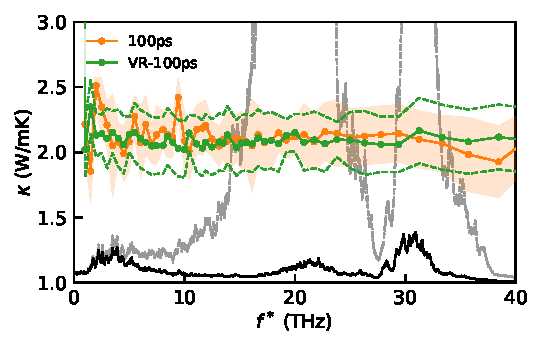
\includegraphics[width=8cm]{chapters/chapter6/figures/silica_expdens_kappa_fstar_VR_100ps.pdf}}
    \subfigure[\label{fig:csilica-sample-expdens-fstar-1ns}]{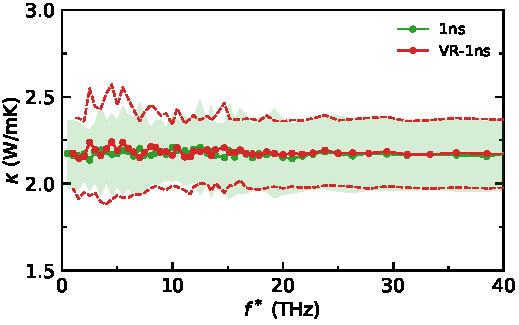
\includegraphics[width=8cm]{chapters/chapter6/figures/silica_expdens_kappa_fstar_VR_1ns.pdf}}
    \subfigure[\label{fig:csilica-sample-expdens-fstar-10ns}]{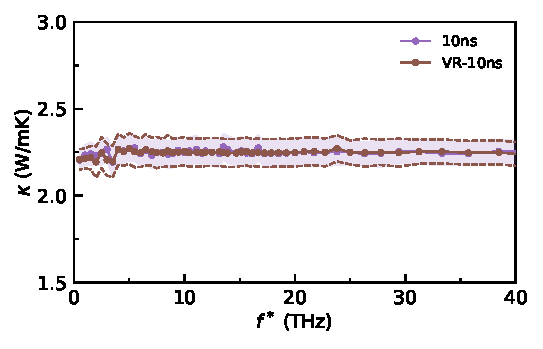
\includegraphics[width=8cm]{chapters/chapter6/figures/silica_expdens_kappa_fstar_VR_10ns.pdf}}
    \caption{Dependence of $\kappa$ on the choice of the cutoff frequency $f^*$, estimated from \emph{one} sample of (a) $100\un{ps}$, (b) $1\un{ns}$, and (c) $10\un{ps}$ of the ``original'' and VR heat flux time series. 
    The original and VR periodograms are reported for reference with grey and black lines, respectively.}
    \label{fig:csilica-sample-expdens-fstar}
\end{figure}
Fig.~\ref{fig:csilica-sample-expdens-fstar} -- stability of $\kappa$ as a function of $f^*$ increases with the length of the trajectory, as its predicted error decreases. The values and errors of $\kappa$ obtained from the VR time series are equivalent to the ones obtained from the original time series, and are slightly more stable with $f^*$. This is probably due to the much smaller power of the power spectrum of the VR heat flux, that may decrease the small artifacts introduced by the low-pass filter applied before resampling. 
Any frequency in the central region of the spectrum can be taken as $f^*$, hence we choose to set $f^*=28\un{THz}$. Conversely, a $f^*$ too small makes $\kappa$ deviate sensibly, due to the fact that the low-pass filter is not strong enough to avoid aliasing effects that modify the spectrum of the resampled time series; instead, a $f^*$ that is too high ($f^*\gtrsim 60\un{THz}$) induces a bias in $\kappa$, due to the fact the log-periodogram diverges to negative values and we start to have problems of numerical precision.

